\chapter{A Quick Overview of Orientation}

This chapter will give a global overview of the necessary tools 
to orientate a set of images.


\label{Intro:QuickApero}

%-------------------------------------------------------------------
%-------------------------------------------------------------------
%-------------------------------------------------------------------

\section{General Organization of Apero}

\subsection{Input and Output}

Apero is a software for computing orientation, position and calibration 
of a set of images compatible with a set of observations, these
obvservations being noisy and (hopefully) highly redondant.
The objective is that you provide the observations,
the confidence you have in these observations, and that
Apero computes the most compatible  solution with your
observations. As the computation of the
optimal solution may be complicated, you will sometimes
have to help and guide Apero.

Basically, the observations can be:

\begin{itemize}
    \item  tie points; in fact, for object modelization it is current that
           the only observations are homologous points;

    \item  ground points;

    \item  observations about the position of the projection center (with GPS embedded in the camera);

    \item  results of previous computation;

\end{itemize}

The confidence you have in the observations is communicated to Apero via weighting functions.

The output of Apero is represented by the computed values of the unkowns,
which can be:

\begin{itemize}
    \item  values of  orientation and position of camera;

    \item  values of  internal calibration;

    \item  values of  ground points coordinates if they are unknown;

    \item  values of  parametric surfaces (still largely undeveloped).

\end{itemize}

% - - - - - - - - - - - - - - - - - - - - - - - - - 

\subsection{General Strategy}

The problem of finding the solution  to orientation is classically divided
into two main sub-problems:


\begin{itemize}
    \item  computation of initial values, hopefully closed to the "real" solution,
           with direct algorithms;
           
    \item  once a reasonable solution is obtained, refine this solution by iteration of :
            \footnote{in photogrammetry, this classical second step has some particularities and it is called bundle adjustment}


\begin{itemize}
       \item linearization of the equations;
       \item solving the redundant linearized equations by some kind of weighted least mean squares;
\end{itemize}
 
\end{itemize}

The first step is the most difficult because there is no known algorithm
for computing directly  a set of orientations compatible with tie points.
There exist several algorithms for computing the relative orientation between
pair of images and these algorithms have to be called many times to build
step by step the global orientation of a large block of images; 
although there is no better known solution,
this incremental approach has two consequences:

\begin{itemize}
   \item  it creates the need of a "good" ordering of the images;
           this order can be specified by the user, or you can let Apero use its
           own heuristics; 

   \item   because the direct algorithms do not use all the information, there is an accumulation
           of errors that can lead to divergence when the refinement step begins; to avoid
           this problem, we have to mix the initialization phase with the refinement phase;

\end{itemize}



The difficulty of the orientation problem is that, to our knowledge, there is no
universal global solution; there is a bag of elementary solutions, and in most cases,
it is possible to assemble these small pieces of solution to build a coherent puzzle.
Practically, there is a lot of current cases, where the orientation can be solved
with a limited number of predefined strategies, and some few cases that
require a very special \UNCLEAR{tuning}. 
What I tried to do when conceiving Apero was to have a tool that simultaneously
gives a fine control to the user, for solving some difficult cases~\footnote{maybe
after some testing}, and that on the other hand offers the possibility to have
predefined files for most current configurations.

The interface \UNCLEAR{around} Apero generally lets the user select one of the predefined
configuration \UNCLEAR{and} %qu'est ce qu'il y a après and?  
Here is an example of predefined strategy currently employed in the
interface developed by Isabelle Clery:




\begin{itemize}

    \item Unknowns: position and orientation of each image, internal calibration common to all images; 
            initially all the internal parameters are frozen; 

     \item        Add the first image, in arbitrary position;

      \item        Iterate: %1- choice the best images to add  by computing stability estimator on the cloud of tie points 
            %2- use the tie points to compute the initial value of the orientation of new image with direct algorithms  
            %3- make one round of a bundle adjustment to avoid error accumulation;
\begin{enumerate}
	\item choose the best images to add  by computing stability estimator on the cloud of tie points;
	\item use the tie points to compute the initial value of the orientation of new image with direct algorithms;
	\item make one round of a bundle adjustment to avoid error accumulation;
\end{enumerate}

       \item      Release one by one the internal parameters in this order : distortion coefficient, focal length, 
            distortion centre, principal point; each time a parameter is released, make a bundle adjustment round;


        \item      Make several rounds of bundle adjustment with more and more strict weighting on the residual of projection.
\end{itemize}


% - - - - - - - - - - - - - - - - - - - - - - - - - 
%-------------------------------------------------------------------
%-------------------------------------------------------------------
%-------------------------------------------------------------------

\section{A First Example}

At first, we will see examples where the ordering is
fixed by the user; although this will be quite uncommon in practicle
case, it is an occasion to understand what it is done by Apero in
the ordering process.

\subsection{Introduction}

The file {\tt Apero-0.xml} is our very first example of using Apero.
To keep it simple we have only two input images. We suppose the camera
is already calibrated, and we try to compute the orientation
of the second image relatively to the first. At the end we output the result
in {\tt XML files}. As in all relative orientation problems, the solution
is \UNCLEAR{undertined} up to a global rotation-translation and scaling, so we will have to
take some action to avoid degeneracy. There are different ways to do it, here we will
fix seven arbitrary values:

\begin{itemize}
  \item  fix the position and orientation of an abitrary pose;
  \item  fix the length of the base between two arbitrary poses.
\end{itemize}





The skeleton of this file is:

{\scriptsize
\begin{verbatim}
  <ParamApero>
       <SectionBDD_Observation>
              ....
       </SectionBDD_Observation>

       <SectionInconnues>
             <CalibrationCameraInc>  ... </CalibrationCameraInc>

             <PoseCameraInc>  .. </PoseCameraInc>
             <PoseCameraInc>  .. </PoseCameraInc>
       </SectionInconnues>

       <SectionChantier> </SectionChantier>
       <SectionSolveur> </SectionSolveur>


       <SectionCompensation>
              <EtapeCompensation> ..  </EtapeCompensation>
              <EtapeCompensation> ..  </EtapeCompensation>
              <EtapeCompensation>  .. 
                     <SectionExport> ... </SectionExport>
              </EtapeCompensation>
       </SectionCompensation>
  </ParamApero>


\end{verbatim}
}

A few comments on the different sections:

\begin{itemize}
       \item {\tt <SectionBDD\_Observation>} contains all the information 
             relative to the observations, this is essentially a set of files
             Apero has to load;

      \item  {\tt <SectionInconnues>} contains the declaration of the
             unknwons and the information necessary to their initialization;

      \item  {\tt <SectionChantier>} and {\tt <SectionSolveur>} contain some possible
             global fine controls of the process, essentially used for internal development;

       \item  {\tt SectionCompensation} contains information for controlling the
              optimization process, essentially weighting of equations, frozing de-frozing
              of unknowns and also \UNCLEAR{generation} of results in the  included {\tt <SectionExport>}.
\end{itemize}

\subsection{Tie Points}

\label{Tie:Poi:Ex:Apero}

Here, the observations are limited to a set of tie-points. The tie points 
we will use are located in the directory {\tt Homol/}. Here, they have been
generated using the tool {\tt Tapioca} described in~\ref{Tapioca}. If you
take a look at the content of {\tt Homol/} you will see that it contains
many subdirectories; go, for example, in {\tt PastisIMG\_5588/}.
It contains many files. Open, for example, {\tt IMG\_5589.txt},
you will see something like:

{\scriptsize
\begin{verbatim}
184.003000 196.441000 43.183200 190.975000
186.997000 222.827000 45.956300 214.604000
188.920000 255.417000 46.587800 245.838000
195.034000 340.312000 50.586800 326.498000
193.219000 246.304000 51.661800 237.330000
194.059000 258.730000 52.074900 249.161000
192.173000 196.095000 52.216800 189.605000
....
\end{verbatim}
}

The structuration of the tie points is probably clear now:
the file {\tt Homol/PastisIMG\_5588/IMG\_5589.txt} contains
the tie points between images {\tt IMG\_5588.txt} and {\tt IMG\_5589.txt}.
This is an ASCII-file, each line contains a tie point in format $x_1 y_1 x_2 y_2$
where $x_1 y_1$ is in {\tt  IMG\_5588.txt} and $x_2 y_2$ is in {\tt  IMG\_5589.txt} .
This structuration should make it easy, if you have a tie point 
generator \UNCLEAR{prefered} to {\tt Tapioca}, to replace it by your own tie points.


Although this structuration is quite evident for human, it has
to be \UNCLEAR{precised} when \UNCLEAR{speaking} to a computer.

\subsection{Declaring the Observations}

The  observation section is:

{\scriptsize
\begin{verbatim}
  <SectionBDD_Observation>
             <BDD_PtsLiaisons>
                 <Id>    Id_Pastis_Hom  </Id>
                 <KeySet> NKS-Set-Homol@@txt  </KeySet>
                 <KeyAssoc>  NKS-Assoc-CplIm2Hom@@txt     </KeyAssoc>
             </BDD_PtsLiaisons>
  </SectionBDD_Observation>

\end{verbatim}
}

Here, as said before, we only have tie-points observations.
They are contained in tags  {\tt BDD\_PtsLiaisons}.
The meaning of the three tags of  {\tt BDD\_PtsLiaisons} is:

\begin{itemize}
    \item {\tt Id} is a name, or identifier, that is given to this set
          of tie points, it will be used each time we will refer to this set;
          it is necessary, because in some special cases, you may have several
          sets of tie points~\footnote{for example, a set computed automatically 
          and a set created by operator} and you will need to indicate the set 
          you are refering to;

    \item  {\tt KeySet} tells Apero  which files of tie points are to be
           loaded, this is a key that refers to a set of files;
           it is detailed below;

    \item  {\tt KeyAssoc} describes to Apero the association that, given
           two image names, can be computed the tie points' file name, and the reverse
           association: given the tie points' file name, how the two images names can be computed;
           examples of names association have already be seen in~\ref{FIRSTASSOC:LOC} (local definition)
            and ~\ref{SECASSOC:PRED} (predefined parametrized key)
           here there are slight innovations and they are described below;
\end{itemize}

The value of {\tt KeySet} is {\tt NKS-Set-Homol@@txt}. This is a predefined key,
its definition can be found in 
{\tt DefautChantierDescripteur.xml}\footnote{directory include/XML\_GEN/}:


{\scriptsize
\begin{verbatim}
    <KeyedSetsOfNames >
          <IsParametrized>  true </IsParametrized>
          <Sets>
                 <PatternAccepteur> Pastis(.*)/(.*)\.(#2)  </PatternAccepteur>
                 <SubDir>   Homol#1/ </SubDir>
                 <NivSubDir> 2 </NivSubDir>
          </Sets>
          <Key> NKS-Set-Homol </Key>
    </KeyedSetsOfNames>
\end{verbatim}
}

This is a parametrized key. Here, the first argument, {\tt \#1}, is empty and 
the second argument, {\tt \#2}, is {\tt txt}.
It describes that the files are in the directory {\tt Homol/}, in the sub-directories {\tt Pastis.*/},
and they have {\tt txt} as a suffix.


The value of {\tt KeyAssoc} is {\tt NKS-Assoc-CplIm2Hom@@txt}.
The definition in {\tt DefautChantierDescripteur.xml} is:

{\scriptsize
\begin{verbatim}
    <KeyedNamesAssociations>
        <IsParametrized>  true </IsParametrized>
        <Calcs>
            <Arrite>  2 1 </Arrite>
            <Direct>
                <PatternTransform> (.*)%(.*) </PatternTransform>
                <CalcName> Homol#1/Pastis$1/$2.#2  </CalcName>
                <Separateur > % </Separateur>
             </Direct>
             <Inverse>
                <PatternTransform> Homol#1/Pastis(.*)/(.*)\.#2 </PatternTransform>
                <CalcName> $1  </CalcName>
                <CalcName> $2  </CalcName>
             </Inverse>
        </Calcs>
        <Key>  NKS-Assoc-CplIm2Hom </Key>
        <SubDirAutoMake> Homol#1 </SubDirAutoMake>
        <SubDirAutoMakeRec> true </SubDirAutoMakeRec>
    </KeyedNamesAssociations>
\end{verbatim}
}

Although we have already seen some examples of key association, there are
some interesting inovations:

\begin{itemize}
   \item  the tag {\tt Arrite} which has the value $2 , 1$. This tag is ignored by the program
          for now, but it is useful for the user.
          $S$ being the set of strings, this tag means  that this key is a mapping $S\times S\rightarrow S$,
          because what we need is to transform the pair of names of images in the name of
          the associated tie points file;

   \item  in {\tt <Cals>}  there is a {\tt <Direct>} and a {\tt <Inverse>}
          part. This is because what we want here is a reversible mapping, {\tt <Direct>} 
          is a $S\times S\rightarrow S$ mapping and {\tt <Inverse>} has to be the $S\rightarrow S\times S$ 
          invers mapping of  {\tt <Direct>}. Apero will need to get back
          the pair of images from the name of the tie points; of course, it is your responsability
          to have the \UNCLEAR{property} that {\tt <Inverse>}  and  {\tt <Direct>} are inverse
          of each other;

    \item {\tt <Direct>} specifies a $S\times S\rightarrow S$ mapping. When it is used, for example, with
          {\tt IMG\_5588.tif}  and {\tt IMG\_5589.tif}, the string {\tt IMG\_5588.tif\% IMG\_5589.tif}
          which matches the regular expression {\tt  (.*)\textbackslash.tif\}\%(.*)\textbackslash.tif};
        
    \item  {\tt <Inverse>} specifies a $S\rightarrow S\times S$ mapping. This is simply
           done by having several {\tt  <CalcName>}, the first {\tt  <CalcName>} specifies
           the first string , the second {\tt  <CalcName>} specifies
           the second string \dots 

\end{itemize}

\subsection{Declaring the Unknowns, Camera-calibration}

The section {\tt SectionInconnues} contains the declaration of the 
unknowns and their initialization. Here, the unknowns are camera
calibration and camera poses.

In this file there is only one calibration. It is declared as:

{\scriptsize
\begin{verbatim}
            <CalibrationCameraInc>
                   <Name> TheKeyCalib   </Name>
                   <CalValueInit>
                       <CalFromFileExtern>
                           <NameFile>   Calib-F050.xml   </NameFile>
                           <NameTag>    CalibrationInternConique </NameTag>
                       </CalFromFileExtern>
                   </CalValueInit>
              </CalibrationCameraInc>
\end{verbatim}
}

The signification of the tags is:

\begin{itemize}
   \item {\tt <Name>} is an identifier that must  be used when refering to this calibration
         \footnote{it would have been more homogeneous to call it {\tt Id} };

   \item {\tt <NameFile>} is the name of the file where Apero will look for
         the initial value of calibration. Take a look at the file {\tt Calib-F050.xml},
         you will understand that it is a typical file for radial distorsion model;

   \item {\tt <NameTag>} is the name of the tag containing the calibration (may be useful,
         for example, if a file contains several calibrations).
\end{itemize}



% - - - - - - - - - - - - - - - - - - - - - - - - - 


\subsection{Declaring the Unknowns, Camera-poses}

There are two pose declarations. The first one is:
{\scriptsize
\begin{verbatim}
            <PoseCameraInc>
                   <PatternName>    IMG_5588.tif   </PatternName>
                   <CalcNameCalib>  TheKeyCalib </CalcNameCalib>
                   <PosValueInit>
                       <PosId> ### </PosId>
                   </PosValueInit>
             </PoseCameraInc>
\end{verbatim}
}

The signification of the tags is:

\begin{itemize}
   \item {\tt <PatternName>} is the pattern of the name of the camera. Here
         it \UNCLEAR{creates} a single camera, but more sophisticated regular expression
         may create multiple \UNCLEAR{creations};

   \item {\tt <CalcNameCalib>} defines the calibration associated to this pose,
         it must be an already created id;

    \item {\tt <PosValueInit>} is the initialization part. It can contain
          different sub-tags, according to the selected initialization method;
         
    \item {\tt <PosId>} means that we want an identity pose 
          \footnote{rotation matrix=identity, centre =$(0,0,0)$};
           in fact, as it is the first image, the value being $100\%$ arbirtrary,
           identity is not a bad choice.
            
\end{itemize}


For the initialization of the second image, we must compute
a rotation coherent with the tie points:


{\scriptsize
\begin{verbatim}
              <PoseCameraInc>
                   <PatternName>     IMG_5589.tif </PatternName>
                   <CalcNameCalib>  TheKeyCalib </CalcNameCalib>
                   <PosValueInit>
                        <PoseFromLiaisons>
                             <LiaisonsInit>
                                 <NameCam> IMG_5588.tif  </NameCam>
                                 <IdBD> Id_Pastis_Hom  </IdBD>
                             </LiaisonsInit>
                        </PoseFromLiaisons>
                   </PosValueInit>
              </PoseCameraInc>
\end{verbatim}
}

The signification of the new tags is:

\begin{itemize}
   \item {\tt <PoseFromLiaisons>} indicates that we initialize with tie points;
   \item {\tt <LiaisonsInit>} indicates that we want to compute the orientation
         of this image, relatively to {\tt IMG\_5588.tif}, the tie points
         being extracted from the {\tt Id\_Pastis\_Hom} set.
\end{itemize}

% - - - - - - - - - - - - - - - - - - - - - - - - - 

\subsection{Running the Compensation}

\subsubsection{What Is Done During the Compensation}

There is no place here to explain in detail what is a bundle adjusment.
We encourage  the interested  reader to consult a book
on the topic.  We just recall, quickly and approximately,
the very basic necessary to understand the control mode
detailed after.

The basic idea is:

\begin{itemize}
   \item let $R_i,C_i$  be the uknown  rotations and position centres;
   \item let  $I_k$ be the unknown intrinsic parameters, with $k=k(i)$;
   \item let  $P_l$ be the unknown ground points corresponding to tie points,
         and $p_{l,m}$ the pixel position of $P$ in the different image where
         it is seen;
   \item note $\pi(R_i,C_i,I_{k(i)},P)$   the projection function;
\end{itemize}

The orientation problem is to find $R_i,C_i$ and $I_k$ (and consequently $P_l$)
so that:

\begin{equation}
     \forall l,m \;   p_{l,m} =  \pi(R_{i(l,m)},C_{i(l,m)},I_{k(i(l,m))},P_l) \label{FORM:IM}
\end{equation}

Generally the problem is redundant, and  equation~\ref{FORM:IM} cannot
be satisfied completely, so we rather search for \UNCLEAR{d} $R_i,C_i$ ,$I_k$ , $P_l$
minimizing the global energy:

\begin{equation}
        res(l,m) =  p_{l,m} -  \pi(R_{i(l,m)},C_{i(l,m)},I_{k(i(l,m))},P_l) \label{FORM:EL2}
\end{equation}

\begin{equation}
      E = \sum_{l,m}  || res(l,m)||^2 \label{FORM:EL2}
\end{equation}

If the equations were linear, and the observations robust, it would be easy:
just run a least mean squares minimization. As the problem is not linear,
Apero classically linearizes the equation for you~\footnote{so this is a Gauss-Newton descent}.
 This is fine but:

\begin{itemize}
   \item  this means  that you will need several iterations;
   \item  there is a risk of divergence if you start too far from the solution;
   \item  there is a risk of divergence if the system has to estimate poorly determined unknowns,
          so you will need a way to freeze, temporarily or not, some unknowns.
\end{itemize}

The classical problem with this quadratic expression is that it gives far too much
importance to outlayers. It is then much more robust to do what is called
$L_1$ minimization:

\begin{equation}
      E = \sum_{l,m}  || res(l,m) || \label{FORM:EL1}
\end{equation}

As $L_1$ minimization is hard to compute directly and \UNCLEAR{very large system}~\footnote{and $L_1$
is not the best solution}, we solve a weighted least mean squares:

\begin{equation}
      E = \sum_{l,m}  \rho(res(l,m)) || res(l,m) ||^2  \label{FORM:ELP}
\end{equation}

The weighting function $\rho$ plays  a very important role, in the solution, and the
convergence itself.  Theoretically $\rho(x)=\frac1x$  leads to $L_1$, a solution already very,
very close to the \UNCLEAR{solution}. %final solution? wanted solution?
Pratically it can lead very easily to divergence \dots
So it is generally prefered to have parametrized weighting functions:


\begin{equation}
   \label{EQ:L1:SEC}
   \rho(x)_{B,\sigma} = if (x>B) \; 0 \; else \;  \frac1{\sqrt{1+(\frac{x}\sigma})^2}
\end{equation}


The problem is to get the good value of $B$ and $\sigma$ \UNCLEAR{?} When we are far from
the solution, as the residual may be high, $B$ and  $\sigma$ must have high values;
then when we get closer and closer, they can have stricter values. The question
is how do you know that you are far or close to the solution. Unfortunately,
I do not know the good answer.

To conclude, the problem of choosing which parameters are to be frozen or
defrozen, and which weighting function is to be used, is a delicate problem
and it will be your problem. Apero will not make the choice for you, but
it will offer, I hope, a fine control on all these options.
This said, what is done during compensation is no more that a weigthed
constraint Gauss-Jordan minimization using \emph{your} parameters for
weitghting and constraining.


%\sqrt{1+\frac{x}\sigma}

\subsubsection{Structure of {\tt SectionCompensation}}

As it can be seen in  file {\tt Apero-0.xml}, the structure is 
the most complicated:

\begin{itemize}
   \item the compensation is made of several  {\tt <EtapeCompensation>},
         for each one you redefine completely the observations and
         their weighting in the {\tt <SectionObservations>};

   \item  each  {\tt <EtapeCompensation>} is made of several  
         {\tt <IterationsCompensation>};

    \item for each  {\tt <IterationsCompensation>}, Apero will
     run a Gauss-Jordan iteration: 

\begin{itemize}
      \item computation \UNCLEAR{of linearised of equation} and accumulation
            in the weighted least squares system;

      \item resolution of least squares system;

      \item update of unknowns with previous solutions;
\end{itemize}

    \item for each  {\tt <IterationsCompensation>}, you have the
          opportunity to freeze of free the unknowns you wish.
\end{itemize}


\subsubsection{Handling the Constraints}

In this example, the constraints are handled very simply,
because they are set at the first iteration and never changed after.
The first {\tt  <IterationsCompensation>} is:


{\scriptsize
\begin{verbatim}
      <SectionContraintes>
            <ContraintesCamerasInc>
                  <Val> eAllParamFiges  </Val>
            </ContraintesCamerasInc>

            <ContraintesPoses>
                  <NamePose>   IMG_5588.tif </NamePose>
                  <Val>      ePoseFigee   </Val>
            </ContraintesPoses>

            <ContraintesPoses>
                  <NamePose>   IMG_5589.tif     </NamePose>
                  <PoseRattachement>   IMG_5588.tif </PoseRattachement>
                  <Val>      ePoseBaseNormee   </Val>
            </ContraintesPoses>
      </SectionContraintes>

\end{verbatim}
}

The meaning of the constraints is:

\begin{itemize}
   \item {\tt <ContraintesCamerasInc>} generates constraints on calibration,
         by default it applies to all created calibrations;
         the enumerated value {\tt eAllParamFiges} means that all parameters are frozen;
         this a reasonable choice because %-1- we have used an alreay calibrated
         %camera for initialization -2-however, we cannot make robust self
         %calibration with two images;
\begin{enumerate}
    \item we have used an already calibrated camera for initialization;
    \item however, we cannot make robust self-calibration with two images;
\end{enumerate}

   \item {\tt <ContraintesPoses>} generates constraints on poses, {\tt <NamePose>}
         indicates to which pose it applies;

    \item for the first image, the value {\tt ePoseFigee} means that the pose
          is completely frozen; this freezes the translation and the rotation of the block (six of the
          seven arbitrary parameters);

    \item for the second image, the value {\tt ePoseBaseNormee} means that in
           the evolution of {\tt IMG\_5589.tif} we freeze the
          length of the base to  {\tt IMG\_5588.tif}; this will freeze the 
          scale of the block (and so the seventh arbitrary constraint);
\end{itemize}

All the constraints are enumerated values, they are of type 
{\tt eTypeContrainteCalibCamera}, defined in {\tt ParamApero.xml}.
Formal description of enumerated values can be found in~\ref{Type::Enum}.


\subsubsection{Using Weighted Observations}

In each {\tt <EtapeCompensation>} there is a {\tt <SectionObservations>}.
Here the observations are limited to one set of tie points, the structure
is the same for the three {\tt <EtapeCompensation>}. There is just
the weighting that evolves.  The first one is:

{\scriptsize
\begin{verbatim}
      <ObsLiaisons>
          <NameRef> Id_Pastis_Hom </NameRef>
          <Pond>
              <EcartMesureIndiv>  1.0 </EcartMesureIndiv>
              <Show> eNSM_Paquet     </Show>
              <EcartMax> 100 </EcartMax>
              <SigmaPond> 5 </SigmaPond>
              <ModePonderation> eL1Secured </ModePonderation>
          </Pond>
      </ObsLiaisons>
\end{verbatim}
}

The meaning of the tags is:

\begin{itemize}
   \item  {\tt <Show>} controls the level of detail for the printed messages;
          it is an enumerated value;
   \item  {\tt <EcartMesureIndiv>} is useless here, but when there are several
          observations, possibly heterogeneous, it will allow to control the
          respective influence of each set of measurements, each weight being
          multiplied by $\frac1{Ec^2}$;
   \item  {\tt <ModePonderation>} is an enumeration controlling which weighting
          function is used; the choice {\tt eL1Secured} corresponds to the function
          of the equation~\ref{EQ:L1:SEC};
   \item  {\tt EcartMax} and {\tt SigmaPond} are the two parameters of equation~\ref{EQ:L1:SEC};
          {\tt EcartMax}  for $B$,  {\tt SigmaPond}  for $\sigma$;
\end{itemize}

% - - - - - - - - - - - - - - - - - - - - - - - - - 

\subsection{Understanding the Message}

Run now the command line:

{\scriptsize
\begin{verbatim}
 bin/Apero ../micmac_data/ExempleDoc/Boudha/Apero-0.xml 
\end{verbatim}
}

On the terminal, you will see a lot of messages:

{\scriptsize
\begin{verbatim}
BEGIN Pre-compile
BEGIN Load Observation
BEGIN Init Inconnues
NUM 0 FOR IMG_5588.tif
NUM 1 FOR IMG_5589.tif
BEGIN Compensation
BEGIN AMD 
AMD::NB= 4
END AMD 
RES:[IMG_5588.tif] ER2 1.04921 Nn 100 Of 4335 Mul 0 Mul-NN 0 Time 0.199447
RES:[IMG_5589.tif] ER2 1.05125 Nn 100 Of 4327 Mul 0 Mul-NN 0 Time 0.164516
| |  RESIDU LIAISON MOYENS = 1.05023 pour Id_Pastis_Hom
--- End Iter 0 ETAPE 0

RES:[IMG_5588.tif] ER2 0.308341 Nn 100 Of 4335 Mul 0 Mul-NN 0 Time 0.160701
RES:[IMG_5589.tif] ER2 0.314634 Nn 100 Of 4327 Mul 0 Mul-NN 0 Time 0.160834
| |  RESIDU LIAISON MOYENS = 0.311503 pour Id_Pastis_Hom
--- End Iter 1 ETAPE 0

 .........

RES:[IMG_5588.tif] ER2 0.124029 Nn 99.9769 Of 4335 Mul 0 Mul-NN 0 Time 0.160253
RES:[IMG_5589.tif] ER2 0.13504 Nn 99.9769 Of 4327 Mul 0 Mul-NN 0 Time 0.159912
| |  RESIDU LIAISON MOYENS = 0.129651 pour Id_Pastis_Hom
--- End Iter 2 ETAPE 2


\end{verbatim}
}

Until the line {\tt END AMD} there is nothing very interesting, there
are messages about initialization process, for internal purpose.
The lines beginning with {\tt RES:} may be useful for interpreting the results:

\begin{itemize}
    \item {\tt [IMG\_5588.tif]} is obviously the name of the image;

    \item {\tt [ER2 0.143439]} is the square root of the weighted average of quadratic residuals;
    
    \item {\tt [Nn 99.9769]} is the percentage of residuals that are under {\tt EcartMax};
          it should be over $95\%$, or else it may signify that you have got residuals just
          because you have thrown away high residuals!

    \item {\tt Of 4327} is the number of tie points;
    \item {\tt Mul 0} is the number of multiple points\footnote{points seen in $3$ or more images};
          here, of course, with two images there are none;

    \item {\tt Mul-NN 0} is the number of multiple points having residuals under {\tt EcartMax};

        \item {\tt Time 0.159912} is the time of computation, internal purpose mainly.
\end{itemize}

% - - - - - - - - - - - - - - - - - - - - - - - - - 
\subsection{Storing the Results}

\label{Result:Apero0}

By default, Apero does not save any result. If you want the result
of your computation to be saved, you must create a {\tt <SectionExport>}
inside the {\tt EtapeCompensation}. Your report result will be executed at the end
of the iterations. Here is the example of {\tt Apero-0.xml}:

{\scriptsize
\begin{verbatim}
       <SectionExport>
              <ExportPose>
                    <PatternSel> (.*).tif </PatternSel>
                    <KeyAssoc> NKS-Assoc-Im2Orient@${AeroOut} </KeyAssoc>
                    <AddCalib>  true </AddCalib>
                    <NbVerif>  10 </NbVerif>
                    <TolWhenVerif> 1e-3 </TolWhenVerif>
              </ExportPose>
       </SectionExport>

\end{verbatim}
}

Here we make an export only for the poses. In {\tt ExportPose} we have:

\begin{itemize}
    \item {\tt <PatternSel>}, a regular expression filtering the name of the pose
          we want to export;

    \item {\tt <KeyAssoc>}, a key referencing an association that, for an image name,
            will compute the name of the file where storing the orientation;
            the same key will be directly reusable in {\tt MicMac} for loading;

    \item {\tt <AddCalib>} indicates that, in each file, we also want to add
          the internal calibration.
\end{itemize}

Now take a look at the directory {\tt ../micmac\_data/ExempleDoc/Boudha/Ori-Test-0}.

%-------------------------------------------------------------------
%-------------------------------------------------------------------
%-------------------------------------------------------------------

\section{More Examples}

% - - - - - - - - - - - - - - - - - - - - - - - - - 
\subsection{Adding More Images}

In the file {\tt Apero-1.xml}, we compute the orientation of a block of 
5 images.  The main difference with {\tt Apero-0.xml} is the added
initialization of the three supplementary images:

{\scriptsize
\begin{verbatim}
      <PoseCameraInc>
           <PatternName>     IMG_559[0-2].tif </PatternName>
           <CalcNameCalib>  TheKeyCalib </CalcNameCalib>
           <PosValueInit>
                <PoseFromLiaisons>
                    <LiaisonsInit>
                         <NameCam> IMG_5588.tif  </NameCam>
                         <IdBD> Id_Pastis_Hom  </IdBD>
                    </LiaisonsInit>
                    <LiaisonsInit>
                         <NameCam> IMG_5589.tif  </NameCam>
                         <IdBD> Id_Pastis_Hom  </IdBD>
                    </LiaisonsInit>
                </PoseFromLiaisons>
           </PosValueInit>
      </PoseCameraInc>
\end{verbatim}
}

The line {\tt PatternName} adds three images, {\tt  IMG\_5590.tif, 
IMG\_5591.tif, IMG\_5592.tif}. For these images, two images are 
given for initialization:

\begin{itemize}
   \item {\tt IMG\_5588.tif}, like before, is used to compute the
        initial position using direct algorithm; however, with only
        one image, there is an ambiguity on the length of the base,
        which is perfectly normal for the second image, but not for
        the following ones;

   \item that is why {\tt IMG\_5589.tif} is given, so that Apero can also
         resolve the base ambiguity in initialization. 

\end{itemize}


As there are more than two images, the information on multiple points
becomes relevant:

{\scriptsize
\begin{verbatim}
RES:[IMG_5588.tif] ER2 0.179343 Nn 99.8955 Of 5739 Mul 4434 Mul-NN 4430 Time 0.361473
RES:[IMG_5589.tif] ER2 0.175283 Nn 99.9625 Of 5333 Mul 4081 Mul-NN 4079 Time 0.339617
RES:[IMG_5590.tif] ER2 0.171174 Nn 99.9401 Of 5009 Mul 3604 Mul-NN 3602 Time 0.311397
RES:[IMG_5591.tif] ER2 0.162117 Nn 99.9807 Of 5187 Mul 3718 Mul-NN 3717 Time 0.32216
RES:[IMG_5592.tif] ER2 0.169253 Nn 99.9196 Of 4977 Mul 3827 Mul-NN 3826 Time 0.316134
\end{verbatim}
}

The export section is slightly different, we store the internal calibration
in a separate file and, instead of copying in each external orientation files,
we add a reference to this file:

{\scriptsize
\begin{verbatim}
                    <SectionExport>
                            <ExportPose>
                                <PatternSel> (.*).tif </PatternSel>
                                <KeyAssoc> NKS-Assoc-Im2Orient@${AeroOut} </KeyAssoc>
                                <AddCalib>  true </AddCalib>
                                <NbVerif>  10 </NbVerif>
                                <TolWhenVerif> 1e-3 </TolWhenVerif>
                                <FileExtern> ${OutCalib} </FileExtern>
                                <FileExternIsKey> false </FileExternIsKey>

                            </ExportPose>
                             <ExportCalib>
                                 <KeyAssoc>  ${OutCalib} </KeyAssoc>
                                 <KeyIsName> true </KeyIsName>
                            </ExportCalib>

                    </SectionExport>
\end{verbatim}
}

The new tags are:

\begin{itemize}
   \item {\tt FileExtern} is the name of the calibration file; for the value  we
         use a symbol defined at the beginning of the file;

   \item {\tt FileExternIsKey} means that the value {\tt FileExtern} is the exact
         string to include, or else it would be used as a key for computing the value
         (useful when multiple calibrations are used);

   \item {\tt ExportCalib} generates a calibration file, {\tt KeyAssoc} is the name
         and {\tt KeyIsName} indicates that it is not to be interpreted as a key.
\end{itemize}


Another difference is in constraint handling:

{\scriptsize
\begin{verbatim}
       <ContraintesPoses>
               <NamePose>   0 </NamePose>
               <Val>      ePoseFigee   </Val>
       </ContraintesPoses>

       <ContraintesPoses>
               <NamePose>   1     </NamePose>
               <Val>      ePoseBaseNormee   </Val>
               <PoseRattachement>   0 </PoseRattachement>
       </ContraintesPoses>
\end{verbatim}
}

Instead of referencing the images by their name, they are referenced
by a number (indicating their order in the initialization process).
As these constraints are totally
arbitrary, this can be more convenient as this  part
of the file stays valid whatever may be the set of images.


% - - - - - - - - - - - - - - - - - - - - - - - - - 
\subsection{Computing the Internal Parameters}

Until now, we have used a file {\tt Calib-F050.xml} that contains a
"good" value of internal calibration, so we have not tried to re-evaluate
this value. However, it will happen very often that you do not have
such a value of internal calibration, and you will need to compute it
by yourself.
The file {\tt Apero-2.xml} and {\tt Apero-2-Bis.xml} introduce how internal 
parameters of calibration can be re-estimated in Apero.

The file containing the initial value  of calibration is {\tt CalibInitNoDist.xml}.
Take a look at this file, you will see it is easy to build such a file:

{\scriptsize
\begin{verbatim}
<ExportAPERO>
    <CalibrationInternConique>
        <KnownConv>eConvApero_DistM2C</KnownConv>
        <PP> 704  469 </PP>
        <F> 1956 </F>
        <SzIm> 1409 938 </SzIm>
        <CalibDistortion>
            <ModRad>
                <CDist> 704  469  </CDist>
            </ModRad>
        </CalibDistortion>
    </CalibrationInternConique>
</ExportAPERO>
\end{verbatim}
}

Some comments:

\begin{itemize}
   \item we choose here a radial model; this is generally a good idea when you do not have
         an explicit reason for selecting something more complicated;

   \item {\tt SzIm} is the size of image; you can easily get it by using any image viewer;

   \item {\tt PP} and {\tt CDist} are principal points and distorsion, by default initialize
         at the center of the image;

   \item \UNCLEAR{{\tt F}, the more complicated,  you have to know (using xif meta data for example)
         the $36mm$  equivalent, here it is a $50mm$, so just do $1409*\frac{50}{36}=1956$.}

\end{itemize}

With this initialization,  {\tt Apero-2.xml} just do the same thing as {\tt Apero-1.xml}.
If you run {\tt Apero-2.xml} you will see that, with this poor calibration, the final residuals are higher.
In  {\tt Apero-2-Bis.xml}, you can see the differences in the second  {\tt EtapeCompensation}:

{\scriptsize
\begin{verbatim}
   <EtapeCompensation>

...
        <IterationsCompensation> </IterationsCompensation>

        <IterationsCompensation>
             <SectionContraintes>
                  <ContraintesCamerasInc>
                       <Val> eLiberte_DR1      </Val>
                  </ContraintesCamerasInc>
             </SectionContraintes>
             <Messages>  LIB  DR1 </Messages>
        </IterationsCompensation>
        <IterationsCompensation> </IterationsCompensation>

        <IterationsCompensation>
             <SectionContraintes>
                  <ContraintesCamerasInc>
                       <Val> eLiberte_DR2      </Val>
                  </ContraintesCamerasInc>
             </SectionContraintes>
             <Messages>  LIB  DR2 </Messages>
        </IterationsCompensation>
        <IterationsCompensation> </IterationsCompensation>

        <IterationsCompensation>
             <SectionContraintes>
                  <ContraintesCamerasInc>
                       <Val> eLiberteFocale_1      </Val>
                  </ContraintesCamerasInc>
             </SectionContraintes>
             <Messages>  LIB  FOCALE </Messages>
        </IterationsCompensation>
        <IterationsCompensation> </IterationsCompensation>
....        
   </EtapeCompensation>
....        

\end{verbatim}
}



\begin{itemize}
   \item the value {\tt eLiberte\_DR1} releases the first  parameter of central distorsion;

   \item the value {\tt eLiberte\_DR2} releases the first and second parameters of central distorsion;
         \UNCLEAR{there exists until} {\tt eLiberte\_DR5};

   \item the value {\tt eLiberteFocale\_1} releases the focal length;
   \item the tag  {\tt <Messages>} generates a message on the terminal.

\end{itemize}

Run {\tt Apero-2.xml}  and {\tt Apero-2-Bis.xml}, you will notice
the significant difference in the final values of the residuals.



% a - - - - - - - - - - - - - - - - - - - - - - - - 
\subsection{Automatic Image Ordering}

\label{Apero:Ordering}

Until now, we have orientated a limited set of images. Now, suppose we
want to orientate all the $26$ images of Buddha, we could use the
previous mechanism specifying  for each image on which image
we want to base the initialization. Of course, we should do it
in the right order \dots It would be quickly unmanageable.

{\tt Apero-3.xml} is a first example. We will let Apero
build for us the tree of image initialization. The first
image is initialized as before, the difference is
in the second set:

{\scriptsize
\begin{verbatim}
     <PoseCameraInc>
          <PatternName>    IMG_[0-9]{4}.tif   </PatternName>
          <CalcNameCalib>  TheKeyCalib </CalcNameCalib>
          <MEP_SPEC_MST>
               <Show> true </Show>
          </MEP_SPEC_MST>

          <PosValueInit>
               <PoseFromLiaisons>
                    <LiaisonsInit>
                         <NameCam> ####  </NameCam>
                         <IdBD> Id_Pastis_Hom  </IdBD>
                    </LiaisonsInit>
               </PoseFromLiaisons>
          </PosValueInit>
     </PoseCameraInc>
\end{verbatim}
}

Here we use the {\tt IMG\_[0-9]{4}.tif} to specify that we want
to load all the gray images of Buddha. Then, we use the
tag {\tt MEP\_SPEC\_MST}. That means that we let Apero build
automatically the initialization tree. Remark that in
{\tt LiaisonsInit}, the {\tt NameCam} is given as dummy value,
in fact it will not be used.

Run this file, you will see that it converges to a reasonable
value of residuals.  However, if you look at the intermediate
results, you will see:

{\scriptsize
\begin{verbatim}
...
| |  RESIDU LIAISON MOYENS = 2.95062 pour Id_Pastis_Hom
--- End Iter 0 ETAPE 0
....
| |  RESIDU LIAISON MOYENS = 12.6271 pour Id_Pastis_Hom
--- End Iter 1 ETAPE 0
....
| |  RESIDU LIAISON MOYENS = 2.41104 pour Id_Pastis_Hom
--- End Iter 2 ETAPE 0
....
\end{verbatim}
}

So you can see that the process goes through a phase of very high 
residuals.  The problem is that the direct initialization 
is error prone; with many images there is an accumulation of error
that can lead to a solution far from the optimal one.
Here it has no big consequences, but this may be a
source of divergence. 

To decrease this risk, Apero proposes a mechanism where you can
mix bundle adjustment with initialization: each time you have
made a given progress in initialization process, you ask to run
the bundle adjustment. You can see the slight differences in {\tt  Apero-3-Bis.xml}:

{\scriptsize
\begin{verbatim}
....
    <PoseCameraInc>

....
           <InitNow> false </InitNow>
           <MEP_SPEC_MST>
                           <Show> true </Show>
           </MEP_SPEC_MST>
....
    </PoseCameraInc>
...
    <SectionCompensation>
         <EtapeCompensation>
               <IterationsCompensation>
...
                      <Pose2Init>
                             <ProfMin> [2,4,6] </ProfMin>
                             <Show> true </Show>
                      </Pose2Init>
               </IterationsCompensation>
         </EtapeCompensation>
    </SectionCompensation>
\end{verbatim}
}

The first difference is in {\tt  <PoseCameraInc>}, the tag 
{\tt <InitNow>} value is {\tt false}; this blocks the initialization.
Then in the first {\tt IterationsCompensation} we have {\tt <Pose2Init>},
when Apero gets this tag, it will do that:

\begin{itemize}
   \item   let us call  depth  of an image its distance to the first
           image in the initialization graph;

   \item   {\tt IterationsCompensation} is run once with all the images
           having a depth $\leq 2$, then once with all the images
           having a depth $\leq 4$ \dots then once with all the image
           having a depth $\leq 10$  \dots until all the images are
           initialized.
\end{itemize}

Run {\tt  Apero-3-Bis.xml}, you will see that the residuals do not
go through a high value phase. 


Another way to avoid divergence is to compute a approximate calibration
with a small set  of convergent images, and then use this result as
initial value in the global set.  Run for example {\tt Apero-3-Ter.xml}.





%-------------------------------------------------------------------
%-------------------------------------------------------------------
%-------------------------------------------------------------------

\section{Geo-referencing}

%  - - - - - - - - - - - - - - - - - - - - - - - - 
\subsection{External Initialization}

Until now, we have always build the orientation "from scratch". This way is 
fine when you use "small" terrestrial acquisition. However, there are
several cases where you would like to start with some pose, having
already a given initial value:

\begin{itemize}
   \item when managing large and complicated acquisition, you may have
         different resolutions of images. It will currently be a good strategy to
         orientate first the low resolution images and, in a second step,
         orientate the high resolution images starting from the already orientated images;
        
   \item when you have an \UNCLEAR{instrumental} %inertial measurement 
    system (IMU), that gives reasonable initial values.
\end{itemize}

The {\tt Apero-4.xml} file shows how known orientations can be used as initial 
values:

{\scriptsize
\begin{verbatim}
...
     <SectionBDD_Observation>
....
             <BDD_Orient>
                  <Id>  Or-Init   </Id>
                  <KeySet>  NKS-Set-Orient@${AeroIn} </KeySet>
                  <KeyAssoc>  NKS-Assoc-Im2Orient@${AeroIn} </KeyAssoc>
             </BDD_Orient>

      </SectionBDD_Observation>

     <SectionInconnues>
....
            <PoseCameraInc>
                   <PatternName>    IMG_[0-9]{3}[02468]\.tif  </PatternName>
                   <CalcNameCalib>  TheKeyCalib </CalcNameCalib>
                   <PosValueInit>
                       <PosFromBDOrient> Or-Init </PosFromBDOrient>
                   </PosValueInit>
             </PoseCameraInc>
....
     </SectionInconnues>
....
\end{verbatim}
}

First, the data containing the observation on initial value has
to be declared for \UNCLEAR{loading in the} {\tt  <SectionBDD\_Observation>}.
\UNCLEAR{This declaration is similar to many observation}
\footnote { {\tt BDD\_PtsLiaisons} has already been seen}:

\begin{itemize}
   \item  in {\tt <Id>}, it is declared the identifier that will be used when
         refering to this data;
    \item {\tt <KeySet>} contains the key describing a set of files;
    \item {\tt <KeyAssoc>} contains the key describing  the association
         between a name of an image and a name of an orientation file;

     \item with {\tt \$\{AeroIn\}} being equal to {\tt -Test-3}, 
          we will load results of {\tt Apero-3.xml}.
\end{itemize}

For initializing the cameras, we use {\tt <PosFromBDOrient>} with
the corresponding Id. This example is quite  artificial, because
we use this initialization with the image having an even number, the
odd number being initialized, as before, by  algorithms. However,
it shows what is the mecanism that could be used in a two step orientation
with different resolutions of images.


%  - - - - - - - - - - - - - - - - - - - - - - - - 
\subsection{Scene-based Orientation}

\label{SC:Base:Or}

There are occasions where, although there is no "real" geo-referencing 
information available, one would like to compute an orientation which is coherent with
some physical constraint:


\begin{itemize}

   \item  use some part of the scene, known to define a horizontal plane, to 
          obtain an orientation where the $OZ$ axis is on the "real" vertical (in 
          fact orthogonal to this plane);

   \item  use a line of the scene, known to be on a given direction,  to
          obtain an orientation where the $OX$ axis is pointing North;

   \item  use an object of known size to set the scale of the model
          (until now, all scaling were totally arbitrary).
\end{itemize}

File {\tt Apero-5.xml} illustrates these three operations. 
The first operation is {\tt <BasculeOrientation>}.
In this operation, a set of $3D$ points known to be coplanar are specified,
a "best" plane $P$ is fitted on these points, then one of the  rotation-translation 
transforming the plane $P$ to the plane $Z=0$ is applied:


{\scriptsize
\begin{verbatim}
   <BasculeOrientation >
        <PatternNameEstim>  IMG_5588.tif </PatternNameEstim>
        <ModeBascule>
             <BasculeLiaisonOnPlan >
                  <EstimPl>
                       <KeyCalculMasq>  NKS-Assoc-AddPost@_MasqPlan </KeyCalculMasq>
                       <IdBdl >Id_Pastis_Hom </IdBdl>
                       <Pond>
                            <EcartMesureIndiv>  1.0 </EcartMesureIndiv>
                            <Show> eNSM_Paquet     </Show>
                            <NbMax>   100    </NbMax>
                            <ModePonderation>  eL1Secured </ModePonderation>
                            <SigmaPond> 2.0 </SigmaPond>
                            <EcartMax> 5.0 </EcartMax>
                       </Pond>
                  </EstimPl>
             </BasculeLiaisonOnPlan>
        </ModeBascule>
   </BasculeOrientation>
\end{verbatim}
}


\begin{figure}
\begin{tabular}{||c||}
   \hline \hline
   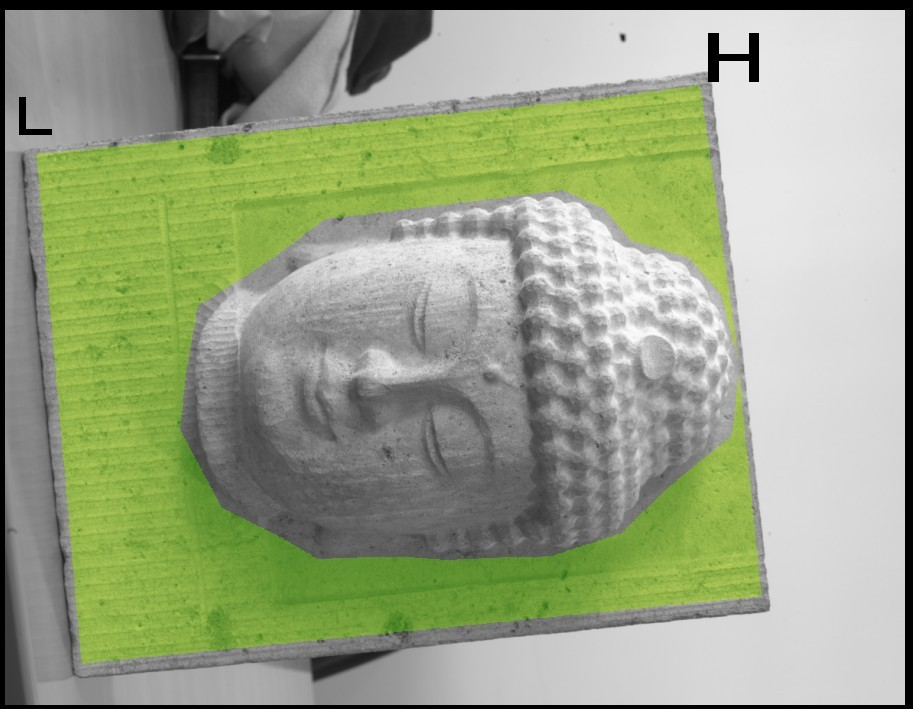
\includegraphics[width=90mm]{FIGS/Boudhas/Masq-Plan-Boudha-Annoted.jpg} \\ \hline  \hline
\end{tabular}
\caption{{\bf Bas Relief} Plane mask used  \dots}
\end{figure}


The meaning of the tags above is the following:

\begin{itemize}
   \item {\tt <PatternNameEstim>} specifies the images $I_k$ that are to be used to
         select the $3D$ points;

   \item for each image $I_k$, {\tt KeyCalculMasq} is used to compute the name 
         of  a file mask $M_k$ (so be careful when setting {\tt <PatternNameEstim>}
         that all corresponding masks exist);


   \item   each tie points $Q$  of  {\tt IdBdl} is selected if,  for at least one
           image, $p$ \UNCLEAR{pf} $Q$, $p$ correponds to one of the $I_k$, and $p$ is
           in the corresponding mask $M_k$; \UNCLEAR{$Q$ is given a weigthing by the
           reprojection ponderation given by} {\tt <Pond>} (of course if the
           weight equals $0$, $Q$ is not selected);   for each selected $Q$,
           the $3D$ point computed by ray-intersection (using current values of pose)
           is added to the point cloud defining the plane.
\end{itemize}

For "small" canvas, it will be generally sufficient to have only one mask for
setting the vertical. However, with linear acquisition, if you want higher precision,
it may be a good idea to have at least two masks, one at the begining and one at
the end.


After  {\tt  <BasculeOrientation>}, the vertical has a physical meaning, but the orientation
is completely arbitrary inside this plane. With the tag {\tt <FixeOrientPlane>},
we can set the "horizontal" orientation:


{\scriptsize
\begin{verbatim}
     <FixeOrientPlane>
          <ModeFOP>
               <HorFOP>
                   <VecFOH>
                       <Pt>  1088 81 </Pt>
                       <Im>  IMG_5588.tif </Im>
                   </VecFOH>
                   <VecFOH>
                       <Pt>  1167 779 </Pt>
                       <Im>   IMG_5588.tif </Im>
                   </VecFOH>
               </HorFOP>
          </ModeFOP>
          <Vecteur>  1 0 </Vecteur>
     </FixeOrientPlane>
\end{verbatim}
}

The idea is to select a  line, and to set its horizontal orientation.
For the most general case, the line  would have to be specified in $3D$ by 
giving two stereoscopic points. This general case will be implemented
later. In the present case, the line is supposed to be horizontal
\footnote{i.e. the points have the same $Z$ after the {\tt <BasculeOrientation>}
has been opered} and two monoscopic points are sufficient, they are transformed into $3D$ points
by giving them the altitude $0$. With this specification,
{\tt Apero} will apply a rotation around the $OZ$ axis so that 
$\overrightarrow{p_1p_2} $ is aligned with $\vec{V}$ \footnote{with $p_1$
and $p_2$ given by {\tt <Pt>} and $\vec{V}$ given by {\tt <Vecteur>}}.


To set the arbitrary scale of the model, a
$3D$ segment of a known size must be specified. To specify a $3D$ segment, 
two stereoscopic points must be specified:


{\scriptsize
\begin{verbatim}
  <FixeEchelle>
         <ModeFE>
              <StereoFE >
                  <HomFE>
                      <P1>193 184 </P1>
                      <Im1> IMG_5588.tif </Im1>
                      <P2> 362 112 </P2>
                      <Im2> IMG_5577.tif</Im2>
                  </HomFE>
                  <HomFE>
                      <P1> 262 869  </P1>
                      <Im1> IMG_5588.tif </Im1>
                      <P2>  473 803 </P2>
                      <Im2> IMG_5577.tif</Im2>
                  </HomFE>
              </StereoFE>
         </ModeFE>
         <DistVraie>  0.2  </DistVraie>
  </FixeEchelle>

\end{verbatim}
}

In the example above, the \UNCLEAR{scaling} %scale
 has been set by specifying that the
height of the rectangle is $20 cm$. For this, the upper left
and lower left corner has been \UNCLEAR{keyed}: each  {\tt <HomFE>} is
the stereoscopic specification of given ground point.


Note that, in the current state of {\tt Apero}'s development, all these transformations
are not made for metrology, they can be used \UNCLEAR{for changing to an orientation having
some sense}, but  they cannot be used during compensation phase.

%  - - - - - - - - - - - - - - - - - - - - - - - - 

\subsection{Using Embedded GPS}

This section treats the case where you have some direction information about
the position of the camera projection center. \UNCLEAR{A current case is with} aerial acquisition
where most systems have a GPS embedded and synchronized with the camera. Of course,
for {\tt Apero} it is just an external information about the summit, and it does not
matter if it comes from GPS of any other system. For simplicity, we will call it
GPS information.

You will generally use this GPS information in two steps:

\begin{itemize}
   \item transform the purely relative orientation computed from tie points 
         to a first geo-referenced orientation;

   \item use this GPS information in the compensation phase by adding a observation
         equation to the global system; of course, as compensation \UNCLEAR{makes} linearization,
         and that linearization requires that you are already close to the solution,
         you cannnot use GPS for compensation before \UNCLEAR{you have made} the global transformation
         described above (that is why it is done in two steps).

\end{itemize}

First, you will  have to attach a center information to each image with which you want
to use this mechanism.
File {\tt Apero-6.xml} illustrates how these operations are made with {\tt Apero}.
In this file, we start from existing relative orientation (read from file),
immediately make the global transformation, and then begin the compensation.
The new parts are:

{\scriptsize
\begin{verbatim}
...
    <BDD_Centre>
          <Id>  Id-Centre   </Id>
          <KeySet>  NKS-Set-Orient@${BDDC} </KeySet>
          <KeyAssoc>  NKS-Assoc-Im2Orient@${BDDC} </KeyAssoc>
    </BDD_Centre>
...
       <SectionInconnues>
             <PoseCameraInc>
....
                   <IdBDCentre> Id-Centre </IdBDCentre>
....
             </PoseCameraInc>
        </SectionInconnues>
....
<SectionCompensation>
              <EtapeCompensation>
                    <IterationsCompensation>
                       <BasculeOrientation>
                          <AfterCompens> false</AfterCompens>
                          <PatternNameEstim> .* </PatternNameEstim>
                          <ModeBascule>
                               <BasculeOnPoints>
                                   <BascOnCentre>   </BascOnCentre>
                                   <ModeL2> true </ModeL2>
                               </BasculeOnPoints>
                          </ModeBascule>
                       </BasculeOrientation>
                    </IterationsCompensation>
....
                   <SectionObservations>
....
                           <ObsCentrePDV >
                              <PatternApply> .* </PatternApply>
                              <Pond>
                                  <EcartMesureIndiv>  1.0 </EcartMesureIndiv>
                                  <Show> eNSM_Paquet     </Show>
                                  <ModePonderation> eL1Secured </ModePonderation>
                              </Pond>
                           </ObsCentrePDV>
....
                    </SectionObservations>
....
              <EtapeCompensation>
</SectionCompensation>
\end{verbatim}
}

The first innovation is the creation of data base of the center {\tt <BDD\_Centre>}.
The mechanism for declaring a set of files, and an association between names 
is the same as usual; each file must contain a tag {\tt  <Centre>}
containing a point in $3D$, see for example {\tt Ori-BDDC/Orientation-IMG\_5564.tif.xml}.

Once the data has been loaded, it must be used to attach a center information
to the images. This is done by  {\tt  <IdBDCentre> Id-Centre </IdBDCentre>}.
In case that not all the images have information center, the 
initialization will have to be split in two {\tt <PoseCameraInc>}.

The global transformation is made by {\tt  <BasculeOrientation>} as in~\ref{SC:Base:Or}.
The parameters are:

  
\begin{itemize}
   \item {\tt <PatternNameEstim>}, it indicates which image must be used. Be warned that, in the
          current version, an error will appear if images without attached center are selected.
          If this pattern does not select at least $3$ images, an error will occur;

   \item  {\tt  <AfterCompens>}, the value {\tt false} specifies that the transformation 
          must be made at the beginning of the {\tt IterationsCompensation} including it. This
          is necessary to insure that the image are geo-referenced when the compensation begins;

    \item {\tt  <BascOnCentre>}, it has no argument, {\tt Apero} knows that the center attached to
          the image must be used;

    \item {\tt <ModeL2>}, it specifies that the global transformation must be made with least mean
          squares optimization.

\end{itemize}


The compensation on the center is made by {\tt <ObsCentrePDV>}. For each selected pose,
the following term is added to the global minimization:


\begin{equation}
       \frac{p(|GPS_k-C_k|) * |GPS_k-C_k|^2}{Ecart^2}
\end{equation}

Where:

\begin{itemize}
    \item $p(|GPS_k-C_k|$ is the usual weighting function; here with no parameters on sigma,
          $p$ values $1$; this is quite common if there is no outlier in GPS;


    \item $Ecart$ for {\tt <EcartMesureIndiv>} allows to control the weighting between 
          heterogeneous measurements (here, the relative importance between tie points and GPS).
\end{itemize}


Note that in this example, we do not use any constraint. This is not necessary for the poses,
because the \UNCLEAR{attach}
 to GPS resolves the scale-translation-rotation ambiguities.
This is not necessary for the internal calibration, because we start from a good initial
value, and there is no risk to \UNCLEAR{free} %release, let free
 all the parameters.



%  - - - - - - - - - - - - - - - - - - - - - - - - 
\subsection{Ground Control Points}

For geo-referencing acquisition ground points are also interesting,
they are generally more precise than embedded GPS and can be acquired in 
\UNCLEAR{more general} condition, on the other hand they are more expensive, time-wise, to
\UNCLEAR{acquired}.

In this section we first describe how the information about ground point
is organized in files so that {\tt Apero} can use them, then we describe
how they can be used in orientation computation.

        %   -    -    -    -    -    -

\subsubsection{Ground Points Organization}

\label{GCP:Org}

The information about ground points will generally be stored in two files:
one for the specification of the points themselves and one for their measurements
in images. In the {\tt Boudha} file take a look at {\tt Dico-Appuis.xml}
and {\tt Mesure-Appuis.xml}. The file {\tt Dico-Appuis.xml} is a list
of declarations of ground points:

{\scriptsize
\begin{verbatim}
<?xml version="1.0" ?>
<Global>
     <DicoAppuisFlottant>
          <OneAppuisDAF>
               <Pt>  103 -645 5</Pt>
               <NamePt>Coin-Gauche </NamePt>
               <Incertitude>  10 10 10  </Incertitude>
          </OneAppuisDAF>
....     
         <OneAppuisDAF>
               <Pt>  370 -544 229 </Pt>
               <NamePt> Levre </NamePt>
               <Incertitude>  10 10 10  </Incertitude>
          </OneAppuisDAF>
     </DicoAppuisFlottant>
</Global>
\end{verbatim}
}

When reading such a file, {\tt Apero} expects to get one object {\tt DicoAppuisFlottant}
which contains a list of {\tt <OneAppuisDAF>}. Each  {\tt <OneAppuisDAF>} specifies:

\begin{itemize}
    \item the value {\tt <Pt>} of the ground point;
    \item the value {\tt <Incertitude>} of the uncertainty associated to each
          point; note that by convention, a value $<0$ on one of the coordinates
          means that this coordinate is totally undefined;
     \item  the value {\tt <NamePt>}, which is an identifier; any string is \UNCLEAR{OK}, %fine
      of course it must be unique.
\end{itemize}

The file {\tt Mesure-Appuis.xml} contains examples of  measurements on
ground points:

{\scriptsize
\begin{verbatim}
<SetOfMesureAppuisFlottants>
     <MesureAppuiFlottant1Im>
          <NameIm> IMG_5576.tif </NameIm>
          <OneMesureAF1I>
               <NamePt> Coin-Gauche  </NamePt>
               <PtIm> 672 218 </PtIm>
          </OneMesureAF1I>
          <OneMesureAF1I>
               <NamePt> Coin-Droite  </NamePt>
               <PtIm> 731 748 </PtIm>
          </OneMesureAF1I>
....
     </MesureAppuiFlottant1Im>
....
</SetOfMesureAppuisFlottants>
\end{verbatim}
}


The signification should be quite obvious:

\begin{itemize}
    \item each {\tt <MesureAppuiFlottant1Im>} contains all the measurements concerning the image
         {\tt <NameIm>};
    \item each measurement contains the name of the point and its position in the image.
\end{itemize}


        %   -    -    -    -    -    -
\subsubsection{Using GCP}

The file {\tt Apero-7.xml} illustrates how GCP can be used:

{\scriptsize
\begin{verbatim}
   <SectionBDD_Observation>
...
       <BDD_ObsAppuisFlottant >
            <Id> Id-Appui </Id>
            <KeySetOrPat>  ^Mesure-Appuis.xml </KeySetOrPat>
       </BDD_ObsAppuisFlottant>
   </SectionBDD_Observation>
   <SectionInconnues>
...
       <PointFlottantInc>
            <Id> Id-Appui </Id>
            <KeySetOrPat>  ^Dico-Appuis.xml$ </KeySetOrPat>
       </PointFlottantInc>
   </SectionInconnues>
...
    <SectionCompensation>
        <EtapeCompensation>
            <IterationsCompensation>
                <BasculeOrientation>
                    <AfterCompens> false </AfterCompens>
                    <PatternNameEstim> .* </PatternNameEstim>
                    <ModeBascule>
                        <BasculeOnPoints>
                             <BascOnAppuis >
                                 <NameRef> Id-Appui </NameRef>
                             </BascOnAppuis>
                             <ModeL2> true </ModeL2>
                        </BasculeOnPoints>
                    </ModeBascule>
                </BasculeOrientation>
            </IterationsCompensation>
...
            <SectionObservations>
                <ObsAppuisFlottant>
                    <NameRef> Id-Appui </NameRef>
                    <PondIm>
                         <EcartMesureIndiv>  1.0 </EcartMesureIndiv>
                         <Show> eNSM_Paquet     </Show>
                         <NbMax>   100    </NbMax>
                         <ModePonderation>  eL1Secured </ModePonderation>
                         <SigmaPond> 20.0 </SigmaPond>
                         <EcartMax> 5000000.0 </EcartMax>
                    </PondIm>
                </ObsAppuisFlottant>
            </SectionObservations>
        <//EtapeCompensation>
    </SectionCompensation>
...
\end{verbatim}
}

First, the GPC and their observations must be loaded:

\begin{itemize}
   \item in the {\tt <SectionInconnues>} they are declared as unknowns in {\tt <PointFlottantInc>},
         their initial value is contained in the file {\tt <KeySetOrPat>};

  \item  in the  {\tt <SectionBDD\_Observation>}, their obsevation in images is loaded;

   \item this is the value {\tt Id-Appui} of  identifier {\tt <Id>}
         that makes the link between unknowns and their observations; it will be used
         further when refering to these GCP.
\end{itemize}

Once the GCP are loaded, they can be used, \UNCLEAR{as GPS}, for a global transformation
or  for compensation once the images are approximatively geo-referenced:

\begin{itemize}
   \item {\tt  <BascOnCentre>} is replaced with {\tt <BascOnAppuis>}, the identifier of
          the GPC set being given as argument; for this operation, there must exist at least
          $3$ GCP being measured in at least $2$ images;


   \item {\tt <ObsCentrePDV>} is replaced with {\tt  <ObsAppuisFlottant>}.
\end{itemize}


In the current version of {\tt Apero}, GPS on summit and GCP cannot be mixed for the
initial global transform. By the way, they can (and often, are) be mixed without
inconvenient in the compensation phase.









